\documentclass[12pt,a4paper]{article}
\usepackage{natbib}
\usepackage{url}
\usepackage{amssymb}
\usepackage{amsmath}
\usepackage{array}
\usepackage{float}
\usepackage{graphicx}
\usepackage{hyperref}
\hypersetup{
	colorlinks=true,
	linkcolor=blue,
	filecolor=magenta,      
	urlcolor=cyan,
}
%titleackage{appendix}
\usepackage[british]{babel}
\bibpunct[:]{(}{)}{;}{a}{,}{,}

%\newcommand{\dd}[1]{\mathrm{d}#1}
\renewcommand{\baselinestretch}{1.5}

\newcommand{\bi}{\begin{itemize}}
	\newcommand{\ei}{\end{itemize}}
\newcommand{\be}{\begin{enumerate}}
	\newcommand{\ee}{\end{enumerate}}

\begin{document}

\begin{titlepage}
	
	\begin{center}
		\textbf{{\Large Draft Paper}}\\
		\vspace{1cm}
		{\Large Pricing a zero coupon bond by Monte Carlo and Finite Difference Methods when the term structure of interest rates is a mean reverting Ornstein-Uhlenbeck process}\\
		\vspace{1cm}
		\today\\
		Valentine Chisango (CHSVAL002)\\
		{\tt vmchisango@gmail.com}\\ 
		
		George Parekkadavil (PRKMAT004)\\
		{\tt gparekkadavil@gmail.com}\\
		
		Vegan Pather (PTHVEG001)\\
		\tt {veganpather@gmail.com}
		
	\end{center}

\begin{abstract}
	Something interesting in this section
\end{abstract}	

\end{titlepage}
\pagenumbering{arabic}
\newpage

\section{Introduction}
\label{sec: Intro}

\newpage
\section{Background}
\label{sec: Backgrd}

The term structure of interest rates provides the relationship between time and interest rates \citep{hull2016options}. This relationship can be modelled by specifying an underlying probability space $(\Omega,\mathcal{F},\mathbb{P})$ as well as a Brownian Motion process $\{W_{s}:t \leq s \leq T\}$ which generates the natrual filtration $\mathbb{F}^{W} = \{\mathcal{F}_{s}^{W}: t \leq s \leq T\}$. A further specification is made for the choice of measure. The common approach for pricing financial instruments is to use the risk-neutral measure $\mathbb{Q}$, which allows for no arbitrage according to the Fundamantal Theorem of Asset Pricing \citep{shreve2004stochastic}. When pricing the zero-coupon bond, the continously compounded interest rate will be modelled as an Ornstein-Uhlenbeck short rate process $\{r_t\}$ and this satisfies the following stochastic differential equation (SDE): 
\begin{equation}
dr_{t} = (\alpha-\beta r_{t})dt + \sigma dW_{t} \quad \alpha, \beta \in \mathbb{R}, \sigma>0
\end{equation}

From this equation, the bond price $B(t,T)$, with boundary condition of $B(T,T) = 1$, can be computed with the following conditional expectation \citep{mamon2004three}.
\begin{equation}
B(t,T) = \mathbb{E}^{\mathbb{Q}}\left[exp\left(-\int_{t}^{T}r_{s} ds\right)\middle\vert\mathcal{F}_{t}\right]
\end{equation}

There are two approaches which can then be used to estimate $B(t,T)$. The first is to use the properties of the Ornstein-Uhlenbeck process, which is proven to have a solution to the SDE which is a Gaussian process \citep{finch2004ornstein}. This means that Normal random variables can be generated over short increments of time and this estimates the integral in (2). This is repeated many times in order to obtain the expected value and this called the Monte Carlo method.

The second approach is to use the partial differential equation (PDE) that is derived from (1) and (2) and the fact that the short rate process obeys the Markov Property \citep{mamon2004three}. The partial differential equation, along with the  boundary condition of $B(T,T) = 1$, is given as follows:
\begin{equation}
-r_t B(t,T) + \frac{\partial}{\partial t} B(t,T) + \frac{\partial}{\partial r_t}B(t,T)(\alpha - \beta r_t) +\frac{1}{2} \sigma^2 \frac{\partial^2}{\partial r_t^2} B(t,T) = 0 
\end{equation}
A series of numerical methods known as finite difference methods are then used to solve this PDE for $B(t,T)$. These methods work by specifying a grid using a discretization of the short rate variable between two values and a discretization of the time variable over $[t,T]$ \citep{ketsise2006monitoring}. These methods start at the maturity time $T$ and approximate the partial differential terms of the PDE at each grid point \citep{crank}. The way in which these terms are approximated vary between the different methods and this leads to salient differences in the resulting bond prices. This paper will make use of different variations of the Monte Carlo method and three finite difference methods in order to approximate the bond price. A more detailed explanation on how these methods are implemented is given in the methodology


\newpage
\section{Methodology}
\label{sec: Method}


\subsection{Monte-Carlo}

We first discretize the SDE using a scheme over a time period [0,T]. The choice of the scheme is between the Euler Marumaya scheme and the Milstein scheme.
	
According to Van Appel, the disretization for the Vasicek model is the same under the Euler or Milstein method. The reason for this being the diffusion term does not depend on $r_t$.  
	
We discretize the model to obtain:
$$ \Delta r_t= (\alpha-\beta r_t)\Delta t+ \sigma \sqrt{\Delta t} z_t+1$$ where $Z_i$
	
$$r_=r_t+\Delta r_t$$ given $r_0$ to be the initial short rate.
	
We then simulate random independent and identically distributed (i.i.d) standard normal variables. These random variables are substituted into the discretized SDE to simulate a path of interest rates.
	
The integral $e^{-\int_{t}^{T} r(u)du}$ is evaluated using one of the paths. This is done by summing up the integrals on one path and then taking its exponential. 
	
This is then repeated for more paths and we take the sample mean as the final estimate of the bond price.
	 
	 


\subsection{Variance reduction techniques}

To decrease the variance of the estimates , three variance reduction techniques will be used. 


\subsubsection{Antithetic variates}

Under this technique, First simulate n i.i.d $Z_i's$ and follow the crude monte carlo technique as above.Repeat the same procedure using  $-Z_i's$.The average of estimates is taken to be the final estimate 


\subsubsection{Moment matching}
The moment matching method, specifically first moment matching, where the sample normal $Z_{i}s$ are transformed to $\hat{Z}_{i}=Z_{i}-\bar{Z}$ where $\bar{Z}=\sum_{i=1}^{n}\frac{Z_{i}}{n}$.

The resulting $\hat{Z}_{i}s$ are not independent and are then used to simulate the short rate values and find the estimates as in the Monte Carlo method.   

 
\subsubsection{Control variates}

Define the price under the close form of the CIR model to be $P_{C}$. Conduct Monte Carlo simulations for the CIR model and define the price under this to be $\hat{P}_{C}$.Conduct Monte Carlo simulations for the Vasicek model and define the price under this to be $\hat{P}_{V}$

Define $P_{V}$ to be the numerical estimate of the bond price

$E[P_{V}]=E[\hat{P}_{V}-\hat{P}_{C}]+P_{V} $

The variance under this method is then:  
\\$VAR[P_{V}]=VAR[\hat{P}_{V}]+VAR[\hat{P}_{C}]-2COV[\hat{P}_{V},\hat{P}_{C}]$ 


    
\subsection{Finite difference method}

The finite difference methods works on a space which is partitioned into a grid by two independent variables. The y variable is the initial rate whilst the x variable is time. A boundary condition exists at time T where the price, B(T,.)=1.The PDE is first discretized .Partial differentials are then calculated at each point on the grid. The bond price is then calculated iteratively at all the grid points by solving for the PDE.

The bond prices are solved for by matrix formulation.    


\subsubsection{Explicit method}

After discretizing the PDE and grouping the similar terms we arrive at the following equation.  

$$B_{i-1,j}=pu_{j}B_{i,j-1}+pm_{j}B_{i,j}+pd_{j}B_{i,j+1}$$ 

where i= 0,....,T \\
      j= $r_0,r_1,....r_n$
      
First we substitute the boundary values into $B_{i,j-1}, B_{i,j}, B{i,j+1}$ and work backwards to calculate the value at point $B_{i-1,j}$ and repeat the process at each point until time t to get the estimates of the prices for varying interest rates $r_0,r_1,...r_n$ 

Note that:       
$$pu_{j}=(r_j/\Delta t)^{-1}(\frac{\sigma^{2}}{2(\Delta r_j)^{2}}+\frac{\alpha-\beta r_j}{2\Delta r_j})$$
$$pm_{j}=(r_j/\Delta t)^{-1}(\frac{1}{\Delta t}-\frac{\sigma^2}{\Delta r_j}^{2})$$
$$pd_{j}=(r_j/\Delta t)^{-1}(\frac{\sigma^{2}}{2(\Delta r_j)^{2}}+\frac{\alpha-\beta r_j}{2\Delta r_j})$$

Under the matrix formulation we have the equation to be:

$$\begin{bmatrix}
	B_{i-1,1} \\
	B_{i-1,2} \\
	\vdots \\       
	B_{i-1,n-1}
	\end{bmatrix}
=
\left( \begin{array}{cccccc}
pm_{1} & pd_{1} & 0 & \cdots  & 0 & 0\\
pu_{2} & pm_{2} & pd_{2} &\cdots & 0 & 0 \\
& pu_{3} & pm_{3} & \cdots & 0 & 0  \\
& \vdots &\vdots & \ddots & \vdots & \vdots \\ 
& 0 & 0 & \cdots & pu_{n-1} & pm_{n-1} \end{array} \right) 
%
\begin{bmatrix}
	B_{i,1} \\
	B_{i,2} \\
	\vdots \\       
	B_{i,n-1}
\end{bmatrix}
+
 \begin{bmatrix}
	pu_{1}B_{i,0} \\
	0 \\
	\vdots \\
	0 \\
	pd_{j-1}B_{i,n-1}
	\end{bmatrix}  
$$
 
 
 
\subsubsection{ Implicit method}

Under this case , once the dicretizationa and grouping of terms occur , we obtain

$$B_{i+1,j}= pu_{j}B_{i,j-1}+pm_{j}B_{i,j}+pd_{j}B{i,j+1} $$

In this case the value at $B_{i+1,j}$ is used to work out the other 3 values. This can be solved simultaneously as when all the equations are written down, there are equal number of equations as to unknowns.


Under this case

$$pu_{j}= (\frac{\alpha-\beta r_{j+1}}{2\Delta r} - \frac{\sigma^2}{2\Delta r^2})\Delta t$$ 
$$pm_{j}= (r_{j+1}+\frac{1}{\Delta t} + \frac{\sigma^2}{\Delta r ^2})\Delta t$$
$$pd_{j}= (\frac{\alpha-\beta r_{j+1}}{2\Delta r} + \frac{\sigma^2}{2\Delta r^2})(-\Delta t) $$

The matrix formulation is:

$$\left( \begin{array}{cccccc}
pm_{1} & pd_{1} & 0 & \cdots  & 0 & 0\\
pu_{2} & pm_{2} & pd_{2} &\cdots & 0 & 0 \\
& pu_{3} & pm_{3} & \cdots & 0 & 0  \\
& \vdots &\vdots & \ddots & \vdots & \vdots \\ 
& 0 & 0 & \cdots & pd_{n-1} & pm_{n-1} \end{array} \right)
%
\begin{bmatrix}
B_{i,1} \\
B_{i,2} \\
\vdots \\
B_{i,n-1}
\end{bmatrix}
=
\begin{bmatrix}
B_{i+1,1} \\
B_{i+1,2} \\
\vdots \\
B_{i+1,r_{n-1}}
\end{bmatrix}
+
\begin{bmatrix}
-pu_{1}B_{i,0} \\
0 \\
\vdots \\
0 \\
-pd_{j-1}B_{i, r_{n-1}}
\end{bmatrix}
$$


\subsubsection{Crank Nicholson}

This method involves making use of $B_{i,j+1}$, $B_{i,j}$ and $B_{i,j-1}$ to evaluate the prices at $B_{i-11,j+1}$, $B_{i-1,j}$ and $B_{i-1,j-1}$. 

$$pu_{j}=\frac{\alpha-\beta r_{j+1}}{4\Delta r} - \frac{\sigma^2}{4\Delta r^2}$$
$$pm_{j}= \frac{\sigma^2}{2 (\Delta r)^2}+\frac{r_{j}}{2}$$
$$pd_{j}=-\frac{\alpha-\beta r_{j+1}}{4\Delta r} - \frac{\sigma^2}{4\Delta r^2}$$

The matrix formulation under this method is:

$$ \left( \begin{array}{cccccc}
-(1/\Delta t)-pm_{1} & -pd_{1} & 0 & \cdots  & 0 & 0\\
-pu_{2} & -(1/\Delta t)-pm_{2} & -pd_{2} &\cdots & 0 & 0 \\
& -pu_{3} & -(1/\Delta t)-pm_{3} & \cdots & 0 & 0  \\
& \vdots &\vdots & \ddots & \vdots & \vdots \\ 
& 0 & 0 & \cdots & -pu_{n-1} & -(1/\Delta t)-pm_{n-1} \end{array} \right
%
\begin{bmatrix}
B_{i-1,1} \\
B_{i-1,2} \\
\vdots \\
B_{i-1,n-1}
\end{bmatrix} 
\\
=
\left( \begin{array}{cccccc}
-(1/\Delta t)+pm_{1} & pd_{1} & 0 & \cdots  & 0 & 0\\
pu_{2} & -(1/\Delta t)+pm_{2} & pd_{2} &\cdots & 0 & 0 \\
& pu_{3} & 1+b_{3} & \cdots & 0 & 0  \\
& \vdots &\vdots & \ddots & \vdots & \vdots \\ 
& 0 & 0 & \cdots & -pu_{n-1} & -(1/\Delta t+pm_{n-1} \end{array} \right) 
%
\begin{bmatrix}
B_{i,1} \\
B_{i,2} \\
\vdots \\
B_{i,n-1}
\end{bmatrix}
+
\begin{bmatrix}
pu_{1}B_{i-1,0} \\
0 \\
\vdots \\
0 \\
pd_{j-1}B_{i-1,n-1}
\end{bmatrix}
+
 \begin{bmatrix}
pu_{1}B_{i,0} \\
0 \\
\vdots \\
0 \\
pd_{j-1}B_{i,n-1}
\end{bmatrix}  
$$


\newpage
\section{Results}
\label{sec: Results}

\subsection{Comparision of Numerical Methods}
\label{subsec: Compar}
The methodology has been implemented in R under an arbitrary set of parameters, where $\alpha = 0.08$, $\beta = 0.8$ and $\sigma=0.005$. This implies a mean rate of 0.10 under the short rate model and an initial rate of 0.08 is selected. These are annually effective and the time to maturity is 5 years. The Monte Carlo methods are all implemented under 1000 trials and with a partition of 200 subintervals over the time range. The partition of time for the finite difference methods was composed of 1250 equally-spaced subintervals, which is consistent with 250 trading days per year. The discrete set of short rates ranged from -0.4 to 0.6 with a step of 0.005. Table 1 provides the corresponding bond prices for each method under these parameters along with the differences between these prices and the known solution. The approximate time to run each method is provided in seconds.



\begin{table}[ht]
\centering
\caption{Comparision of Bond Prices for Numerical Methods}
\vspace{0.5cm}
\label{tab: Table1}
\begin{tabular}{|>{\centering\arraybackslash}m{4.5cm}|>{\centering\arraybackslash}m{2cm}|>{\centering\arraybackslash}m{2cm}|>{\centering\arraybackslash}m{2cm}|>{\centering\arraybackslash}m{2cm}|}
	\hline
	Numerical Method & Price & Known Price & Error & System Time \\ 
	\hline
	Crude Monte Carlo & 0.62114 & 0.62164 & 0.00050 & 0.72 \\ 
	Antithetic Variates & 0.62460 & 0.62164 & -0.00296 & 0.95 \\ 
	Moment Matching & 0.62840 & 0.62164 & -0.00676 & 1.01 \\ 
	Control Variates & 0.62152 & 0.62164 & 0.00011 & 1.33 \\ 
	Explicit Method & 0.62194 & 0.62164 & -0.00031 & 0.1\\ 
	Implicit Method & 0.62193 & 0.62164 & -0.00030 & 0.2 \\ 
	Crank-Nicolson Method & 0.62188 & 0.62164 & -0.00024 & 0.24 \\ 
	\hline
\end{tabular}
\end{table}

\subsubsection{Speed}
The results in \hyperref[tab: Table1]{Table 1} show that the finite difference methods have a significanlty smaller computation time than the Monte Carlo methods. The Crude, Antithetic Variates and Moment Matching methods all show higher error terms than the finite difference methods even though their computation times are higher. However the Control Variates method produces the closest result to the known solution but it also has the highest run time. 



\subsubsection{Convergence}

In terms of the Monte Carlo methods, convergence to the known solution may be achieved as the number of trials increase. \hyperref[fig:MC Conv]{Figure 1} is a depiction of how the results behave as the number of trials increases from 0 to 2000 for each Monte Carlo method. 
\begin{figure}[H]	
	\label{fig:MC Conv}
	\begin{center}
		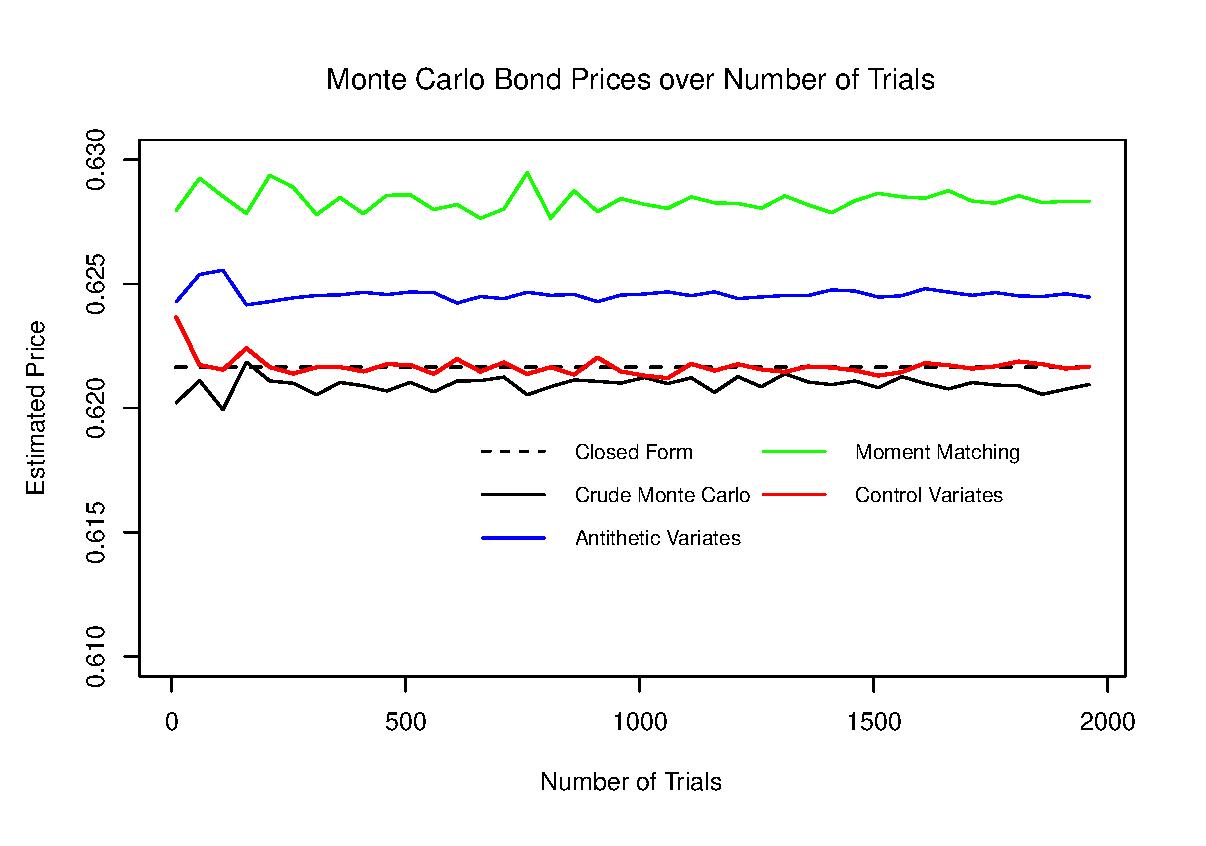
\includegraphics[trim={0 0.5cm 0 0},clip, width = 14cm]{MC_Conv.eps}
		\caption{Convergence of Monte Carlo Bond Prices}
	\end{center}
\end{figure}

All methods show a lack of convergence for smaller trials but the Moment Matching and Antithetic Variates methods demonstrates no clear tendency towards the known solution even for very high trials. The Crude Monte Carlo method demonstrates a closer convergence however the Control Variates method shows the highest convergence to the known solution.

In terms of the Finite Difference methods, convergence can be analysed by observing the methods as the partition of the grid becomes dense. Since maturity time is held constant, the time partition is made to be finer by increasing the number of subintervals. \hyperref[fig:Fig Conv]{Figure 2} shows how the bond price estimates change as the partition of time becomes more dense.
\begin{figure}[H]
	\label{fig:Fig Conv}
	\begin{center}
		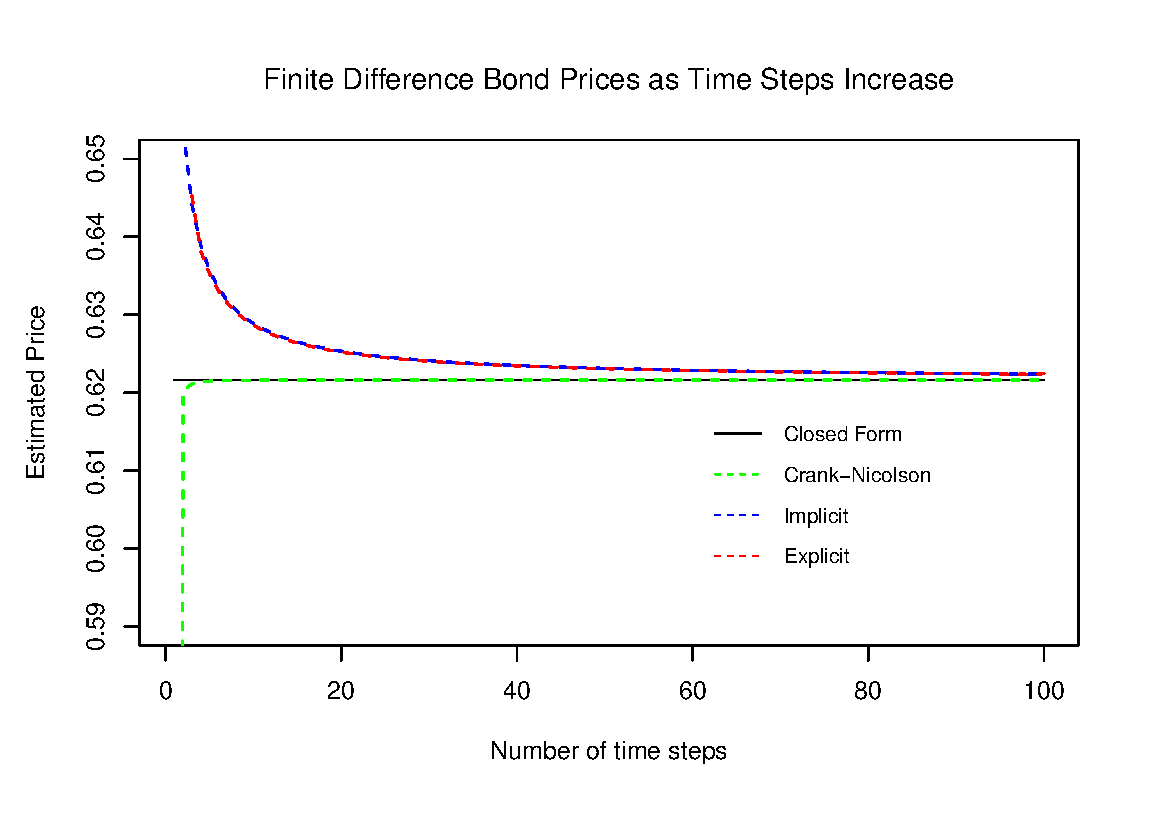
\includegraphics[trim={0 0.5cm 0 0},clip, width = 14cm]{Fin_Conv.eps}
		\caption{Convergence of Finite Difference Bond Prices}
	\end{center}
\end{figure}

All methods tend towards the known solution with the implicit and explicit methods showing a similiar rate of convergence. However, Crank-Nicolson method demonstrates a slower rate of convergence than the other methods.


\subsubsection{Stability}

\subsection{Sensitivy Tests}
In order to confirm that the behaviour of the numerical methods is as expected under different parameters, several different parameter values are tested. The initial set of parameters are those used in section \ref{sec : Compar}. From here the input parameters are varied one at time, with $\alpha$ and $\beta$ varied together in the final two scenarios tested. For each parameter varied, the bond price produced by each numerical method under the chosen scenarios is plotted along with the bond price produced by the closed form solution.
In varying the interest rate from the initial $8\%$, all methods behave as expected. When the interest rate is reduced to $5\%$, the bond price decreases. When the interest rate is raised to $10\%$, the bond price increases.	Varying the time to maturity ($T$) from the initial $5$ years also results in the expected behaviour: bond prices increase when $T=1$ and decrease when $T=10$. However, the bond price produced by the explicit method decreases significantly and is in fact negative. This is caused by [missing].
All the methods behave normally when the standard deviation is increase from the initial $0.5\%$ to $1\%$. When the standard deviation is decreases to $0.1\%$, the Monte-Carlo methods produce slightly lower bond prices while the finite differences produce bond prices in excess of 2. This highlight the flaw in finite difference methods in that they produce very large prices, that don't make financial sense since they exceed the pay-off of the bond, when the standard deviation is sufficiently small and almost vanishes from the partial differential equation from which the tridiagonal matrices used for the methods are created.
In order to confirm that the behaviour of the numerical methods is as expected under different parameters, several different parameter values are tested. The initial set of parameters are those used in section \ref{sec : Compar}. From here the input parameters are varied one at time, with $\alpha$ and $\beta$ varied together in the final two scenarios tested. For each parameter varied, the bond price produced by each numerical method (labelled from 2 to 8 in the order Closed Form,Crude Monte Carlo, Antithetic Variates, Moment Matching, Control Variates, Explicit, Implicit, Crank Nicholson) under the chosen scenarios is plotted along with the bond price produced by the closed form solution (labelled 1).
In varying the interest rate from the initial $8\%$, all methods behave as expected. When the interest rate is reduced to $5\%$, the bond price decreases. When the interest rate is raised to $10\%$, the bond price increases.	Varying the time to maturity ($T$) from the initial $5$ years also results in the expected behaviour: bond prices increase when $T=1$ and decrease when $T=10$. However, the bond price produced by the explicit method decreases significantly and is in fact $-4.873359\times10^{32}$. This is caused by [missing].
All the methods don't result in significant changes to the bond price when the standard deviation is increases from the initial $0.5\%$ to $1\%$. When the standard deviation decreases to $0.1\%$, the Monte-Carlo methods don't see significant changes in bond prices while the finite differences produce bond prices in excess of 2. This highlights the flaw in finite difference methods in that they produce very large prices, that don't make financial sense since they exceed the pay-off of the bond, when the standard deviation is sufficiently small and almost vanishes from the PDE along with its coefficients.
When alpha is decreased from the initial $0.08$, the bond prices for all methods increase. When alpha is increased, the bond prices for all methods decrease, with the price produced by the explicit method again decreasing rapidly to $-1.257679$. When the value of beta is decreased from the initial $0.8$, the bond price produced by all methods decreases. When beta is increases, the bond price produced by all methods increases, which the exception of the explicit. For the explicit method, the price is once again negative and equal to $-2.492100\times10^{45}$. If alpha and beta are varied simultaneously such the mean remains constant and only the mean reversion rate changes then the bond prices don't vary significantly, with the prices being higher for the higher mean reversion rates (i.e. the higher beta value). Again an exception is found with the explicit method, where the price for the increased beta is $-5.065734\times10^{34}$.
\
\newpage
\section{Conclusions}
\label{sec : Concl}



\newpage
\bibliographystyle{natbib}
\bibliography{myref}	

\newpage
\appendix
\section{Appendix A}
\label{sec: Appendix A}
\subsection{Details of the Model}
\label{subsec: Details}
The formulation consists of a zero-coupon bond issued at some time $t \geq 0$ where a corresponding payment of 1 unit will be made at the maturity time $T \geq t$. The risk of default is negligible \citep{shreve2004stochastic}. The bond is priced by using the short rate process $\{r_{s}:t \leq s \leq T\}$.

For the time interval $[t,T]$ the filtered probability space $(\Omega, \mathcal{F}^W,\mathbb{F}^W,\mathbb{P})$ is used and $r_t$ is known \citep{mamon2004three}. A risk neutral measure $\mathbb{Q}$ is defined and it is equivalent to $\mathbb{P}$ \citep{shreve2004stochastic}. The short rate process, which is an Ornstein-Uhlenbeck process, then satisfies the following stochastic differential equation: 
\begin{equation}
dr_{t} = (\alpha-\beta r_{t})dt + \sigma dW_{t} \quad \alpha, \beta \in \mathbb{R}, \sigma>0, \beta \neq 0
\end{equation}


The bond price $B(t,T,r_t)$ with boundary condition of $B(T,T,r_t) = 1$, is then determined through computing the following risk-neutral expectation:
\begin{equation}
B(t,T,r_t) = \mathbb{E}^{\mathbb{Q}}\left[exp\left(-\int_{t}^{T}r_{s} ds\right)\middle\vert\mathcal{F}_{t}^{W_{t}}\right]
\end{equation}


\subsection{The Partial Differential Equation}
\label{subsec: PDE}
The following expression is the PDE, derived from (2), which is required to obtain the price of a zero-coupon bond when the term structure of interest rates follows the Ornstein-Uhlenbeck process. .
$$\boxed{-r_t B(t,T,r_t) + \frac{\partial}{\partial t} B(t,T,r_t) + \frac{\partial}{\partial r_t}B(t,T,r_t)(\alpha - \beta r_t) +\frac{1}{2} \sigma^2 \frac{\partial^2}{\partial r_t^2} B(t,T,r_t) = 0 }$$

\noindent This PDE is accompanied by the boundary condition $B(T,T,r_t) = 1$
\subsection{The Closed Form Solution}
\label{subsec: Closed Form}

A closed form solution to the above PDE exists and as per \cite{mamon2004three}, it is given by the following expression:
\begin{gather*}
\boxed{B(t,T,r_t) =exp(-A(t,T)r_t+D(t,T))}
\end{gather*}
where
\begin{align*}
A(t,T)&=\frac{\beta(1-e^{-\beta(T-t)})}{\alpha}\\
D(t,T)&=\frac{1}{\beta}\left[\left(\alpha-\frac{\sigma^2}{2\beta}\right)[A(t,T)-(T-t)]-\frac{\sigma^2A(t,T)^2}{4}\right]
\end{align*}

\newpage
\section{Appendix B}
\label{sec: Appendix B}
\subsection{Monte Carlo Simulation}
\label{subsec: MC}
The methodology involved in Monte-Carlo simulations are:

\begin{itemize}
	\item Discretize the SDE using a scheme over a time period [0,T]
	\item Simulate random i.i.d standard normal variables.
	\item Simulate a path of interest rates using the discretized SDE and the i.i.d standard normal variables.
	\item Evaluate the integral $e^{-\int_{t}^{T} r(u)du}$ using one simulated path.
	\item Repeat the evaluation for more paths and take the sample mean as the final estimate of the bond price.
	
	The above steps are mentioned in Cairns(2004:185)
\end{itemize}



\subsubsection{Schurman's Method Under the Vasicek Model}
\label{subsubsec: Schurman}

Schurman(2009) determined the following formula as the bond price for one interest rate path with fixed parameters.  

$$f(h,n)=F\times exp[-\{\frac{1}{2}r_{0}+\sum_{j=1}^{k-1}r_{j} +\frac{1}{2}r_{k}\}h]$$

where F is the face value of the bond, h is the time interval, n being the number of the path simulated and $r_{j}$ are the short rate values simulated. Monte Carlo simulations are then run on each path level to determine the price of along that simulated interest rate path. Once N simulations have been completed, the final price is then determined by taking the average of the prices across N simulations.   

\subsection{Finite Difference Methods}
\label{subsec: FD}
A space-time grid (or lattice) is defined by the independent variables of $t$ and $r_t$ \citep{crank}. The interval $[t,T]$ is partitioned into equal sub-intervals with indices of  $n=0,1,...,N$. The range of $r_t$ (which is treated as the space variable) is partitioned with indices of $i = 1,...,I$. The lenght of each $r$ sub-interval is taken as $\Delta r_t$ and the lenght of each $t$ sub-interval is taken as $\Delta t$. The function in the PDE is given by $f(t,r_t)= B(t,T,r_t)$ with boundary condition $f(T,r_t) = 1$ and $r_t$ being known. The algorithm starts at $f(T,r_t)$ works backwards until the solution is reached and this runs over the $(N+1)\times(I+1)$ grid points. At a single gridpoint $(n,i)$, the following approximations are made:
\subsubsection{Explicit Method}
\label{subsubsec: Explicit}
$$\frac{\partial f}{\partial t} = \frac{f(n+1,i) - f(n,i)}{\Delta t}$$
$$\frac{\partial f}{\partial r_i} = \frac{f(n+1,i+1) -f(n+1,i-1)}{2 \Delta r_i}$$
$$\frac{\partial^2 f}{\partial r_i^2} = \frac{f(n+1,i+1) - 2f(n+1,i) +f(n+1,i-1)}{\Delta r_i^2}$$

This is used in the PDE as follows
$$-r_i f(n,i)  + \frac{\partial f}{\partial t} + \frac{\partial f}{\partial r_i}(\alpha - \beta r_i) +\frac{1}{2} \sigma^2 \frac{\partial^2 f}{\partial r_i^2}  = 0 $$

\subsubsection{Implicit Method}
\label{subsubsec: Implicit}
$$\frac{\partial f}{\partial t} = \frac{f(n+1,i) - f(n,i)}{\Delta t}$$
$$\frac{\partial f}{\partial r_i} = \frac{f(n,i+1) -f(n,i-1)}{2 \Delta r_i}$$
$$\frac{\partial^2 f}{\partial r_i^2} = \frac{f(n,i+1) - 2f(n,i) +f(n,i-1)}{\Delta r_i^2}$$

This is used in the PDE as follows
$$-r_i f(n+1,i)  + \frac{\partial f}{\partial t} + \frac{\partial f}{\partial r_i}(\alpha - \beta r_i) +\frac{1}{2} \sigma^2 \frac{\partial^2 f}{\partial r_i^2}  = 0 $$
\subsubsection{Crank-Nicolson Method}
\label{subsubsec: Crank Method}

$$\frac{\partial f}{\partial t} = \frac{f(n+1,i) - f(n,i)}{\Delta t}$$
$$\frac{\partial f}{\partial r_i} = \frac{f(n,i+1) - f(n,i-1) +f(n+1,i+1) -f(n+1,i-1)}{2 \Delta r_i}$$

\begin{gather*}
\frac{\partial^2 f}{\partial r_i^2} = \frac{f(n,i+1) - 2f(n,i) + f(n,i-1)}{2\Delta r_i^2}
+ \frac{f(n+1,i+1) - 2f(n+1,i) +f(n+1,i-1)}{2\Delta r_i^2}
\end{gather*}

This is used in the PDE as follows
$$-\frac{1}{2}r_i f(n,i)-\frac{1}{2} r_i f(n+1,i) + \frac{\partial f}{\partial t} + \frac{\partial f}{\partial r_i}(\alpha - \beta r_i) +\frac{1}{2} \sigma^2 \frac{\partial^2 f}{\partial r_i^2}  = 0 $$

The PDE can then be simplified further which results in solving a tridiagonal system of equations \citep{Cairns}.
	
	
\end{document}
